
\documentclass[12pt]{article}


\usepackage{times}
\usepackage{graphicx}
\usepackage{comment}
\usepackage{amsmath,amssymb}
\usepackage{natbib}

\usepackage{tikz}
\usetikzlibrary{arrows}



\topmargin 0.0cm
\oddsidemargin 0.2cm
\textwidth 16cm 
\textheight 21cm
\footskip 1.0cm



\newenvironment{sciabstract}{%
\begin{quote} \bf}
{\end{quote}}


\renewcommand\refname{References and Notes}


\newcounter{lastnote}
\newenvironment{scilastnote}{%
\setcounter{lastnote}{\value{enumiv}}%
\addtocounter{lastnote}{+1}%
\begin{list}%
{\arabic{lastnote}.}
{\setlength{\leftmargin}{.22in}}
{\setlength{\labelsep}{.5em}}}
{\end{list}}



\title{Generalized Additive Mixed Models for intraspeaker variation} 



\begin{comment}
\author
{Meredith Tamminga,$^{1\ast}$ Christopher Ahern,$^{1}$ Aaron Ecay$^{2}$\\
\\
\normalsize{$^{1}$Department of Linguistics, University of Pennsylvania}\\

\normalsize{$^{2}$Department of Language and Linguistic Science, University of York}\\
\\
\normalsize{$^\ast$To whom correspondence should be addressed: tamminga@ling.upenn.edu}
}
\end{comment}

\date{}



%%%%%%%%%%%%%%%%% END OF PREAMBLE %%%%%%%%%%%%%%%%




\begin{document} 


\baselineskip24pt


\maketitle 

\begin{abstract}
Intraspeaker sociolinguistic variation is typically characterized by repetitiveness in what choices speakers make from moment to moment, but there are multiple possible sources of such repetitiveness. We distinguish two types of temporal clustering: sequential dependence and baseline deflection. We argue that because we have independent reasons from sociolinguistics and psycholinguistics to believe both types are at play in speech production, it is desirable to adopt quantitative models that can simultaneously estimate these distinct sources of temporal clustering. We propose the use of Generalized Additive Mixed Models (GAMMs) for this purpose and illustrate with a case study of DH-stopping in Philadelphia English sociolinguistic interviews. We advocate for the adoption of GAMMs to advance the use of naturalistic data for studying psycholinguistic questions about intraspeaker variation.

\end{abstract}

\section{Introduction} \label{intro}


    
Non-independence of observations is a general problem in quantitative linguistic research \citep{paolillo:2002}. This is especially true for  research using naturalistic data that tries to connect observed intraspeaker variability in spontaneous speech with more carefully-controlled experimental results---connections which might serve both to confirm the real-world operation of psycholinguistic phenomena and to provide sociolinguists and corpus linguists with explanatory mechanisms for  observed patterns of variation. One source of non-independence is the collection of multiple data points per individual, which is of course necessary for the observation of intraspeaker variation. The introduction and uptake of mixed-effects regression \citep{Baayen:2008,Barr:2013} has allowed this type of non-independence to be controlled statistically. The collection of multiple observations from proximal locations is a similar problem in studies of spatially-distributed linguistic variation \citep{Wieling:2014}. In this paper we apply the same tool that has been used to handle geographic non-independence---Generalized Additive Mixed Models (GAMMs)---to a problem of temporal non-independence: that sequential instances of a varying linguistic item in conversational speech are not independent. Instead, temporally proximal instances of a sociolinguistic variable are more likely to surface in the same form than are instances that occur further apart \citep{Sankoff:1978}. 
    
We  distinguish two general classes of mechanisms that can give rise to such temporal clustering. First are what we term \textbf{sequential dependence} mechanisms: those in which the outcome of a sociolinguistic alternation in one moment directly influences the likelihood of a matching outcome some moments later. 
This type of repetitiveness is of psycholinguistic interest because it might arise from one or more sources of psycholinguistic facilitation, such as priming via neural activation or error-driven implicit learning. 
The second source of temporal clustering is what \citet{Tamminga:2016a} call \textbf{externally-motivated baseline deflection}. If we imagine a speaker as having some target probability (a baseline) for their choice between two linguistic alternants, we might expect that target rate to fluctuate over time in response to elements in the real-world setting. Two closely-proximal instances of a sociolinguistic variable are more likely to occur under similar social-contextual circumstances than two instances that are further apart, and thus are more likely to have matching outcomes.
The relationship between sequential dependence and baseline deflection can be summarized visually as in Figure \ref{confounding}, where we consider a sequence of observations of a probabilistic alternation over time. We represent sequential dependence as an arrow from $X_{t-1}$ to $X_t$, indicating the influence of the previous alternant chosen on the next choice made. We represent baseline deflection as an arrow from factor(s) $Y$ to each instance in the sequence of choices.
What factors are represented by $Y$ is an empirical and theoretical question in its own right: just as sequential dependence as a term is intended to cover a range of possible factors, so too is the terminology of baseline deflection intended to capture many disparate elements of how speakers respond in real time to contextual factors.
The social processes by which speakers dynamically navigate conversational demands and discourse context are enormously complex; while Figure \ref{confounding} shows why in principle sequential dependence and baseline deflection are distinct, in practice it has proven difficult to dissociate them in conversational speech data.
Of particular consequence for research on intra- and inter-speaker variation by psycholinguists is that this potential conflation leaves naturalistic studies of psycholinguistic phenomena like  priming vulnerable to the criticism that they are actually capturing something more like style-shifting or discourse coherence \citep{Szmrecsanyi:2006}.
 Our goal is to reduce that complex information to a single abstract dimension in order to make it quantitatively tractable.
In doing so, we aim to provide psycholinguists, sociolinguists, and corpus linguists with a tool to better control a range of potentially-confounding factors when studying psycholinguistic phenomena in naturalistic data.


\begin{figure}
\begin{center}
        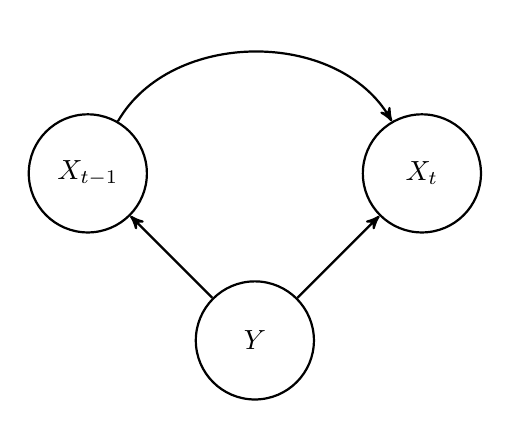
\begin{tikzpicture}[->,>=stealth',auto,node distance=3cm, thick]
	  \node (X) [draw,circle,minimum size=1.5cm]  at (0,0) {$X_{t-1}$};
	  \node (Z) [draw,circle,minimum size=1.5cm, below right of=X]  {$Y$};
	  \node (Y) [draw,circle,minimum size=1.5cm, above right of=Z]  {$X_{t}$};
	  \path[every node/.style={font=\sffamily\small}]
	    (Z) edge node [right] {} (X)
	    (Z) edge node [right] {} (Y)
	    (X) edge[bend left=60] node [right] {} (Y);
	\end{tikzpicture}         
    \end{center}
\caption{The relationship between sequential dependence and baseline deflections in the temporal use of variants}
\label{confounding}
\end{figure}



 
 In this paper we propose the use of Generalized Additive Mixed Models (GAMMs,  \citealt{hastie1990generalized}, \citealt{zhang1999}, \citealt{ruppert2003}) 
 for the simultaneous estimation of sequential dependence and baseline deflection. 
The use of generalized additive modeling is a relatively new but not unknown statistical technique in psycholinguistics; GAMs and GAMMs have been used to model nonlinearities in eye tracking data \citep{Nixon:2016}, EEG measurements \citep{Tremblay:2014,DeCat:2015}, 
and behavioral reaction times \citep{Pham:2013,Feldman:2015}.
We use intraspeaker sociolinguistic variation data drawn from a corpus of conversational interviews to illustrate the application of GAMMs to problems of temporal non-independence. 
 GAMMs, and their non-hierarchical counterparts Generalized Additive Models (GAMs), allow for smooth functions of independent variables to be incorporated into regression models, which is ideal for modeling baseline deflection because for any given conversation, we have no \textit{a priori} expectations about when externally-motivated fluctuations in linguistic behavior should occur. We can thus include in the models smooth functions of time elapsed as a way of capturing baseline deflection in variant rates.  At the same time, we also include a predictor for the value of the previously-occurring observation, which is the usual practice for identifying sequential dependence in naturalistic data. 
Using a GAMM thus allows us to systematically attribute apparent repetitiveness in the linguistic choices speakers make either to the value of the immediately prior choice the speaker made or to overall fluctuations in the speaker's alternant use rate due to contextual shifts. 
After illustrating the specification of both a GAM and a GAMM to capture intra- and inter-speaker sociolinguistic variability, we will discuss possible interpretations of the model components. Our hope is not to answer any particular theoretical question in the current paper, but rather to make some suggestions about how GAMMs could be elaborated to investigate a range of theoretical questions about the real-world dynamics of variation in speech production. 

\section{Background} \label{background}

Baseline deflection and sequential dependence are, as discussed above, cover terms for two classes of mechanisms that may lead to temporal clustering of variation in conversational speech. A brief overview of the empirical research that has observed the existence of such clustering is thus in order.
Of particular relevance is work on a phenomenon that corpus linguistic and sociolinguistic researchers using conversational speech data  sometimes call \emph{persistence} \citep{Szmrecsanyi:2006}: the tendency to repeat a sociolinguistic variant that has recently been used. Research on persistence has emphasized the presumed connection between persistence as observed in conversational speech and \emph{priming} as observed in the laboratory under carefully controlled experimental conditions \citep{Cameron:2004,Gries:2005,Szmrecsanyi:2006,Tamminga:2014b}; as mentioned above, priming may itself be a cover term for different facilitatory mechanisms.
In an experimental psycholinguistic context, priming may manifest as shortened reaction times for lexical access to primed words \citep{Goldinger:1996} or increased use of a primed syntactic structure in production \citep{Pickering:2008}. In naturalistic speech, the facilitatory mechanisms whose effects are observed in the lab are presumably still at work, but identifying them is more difficult given the many factors at play in the production of conversational speech. Nonetheless, it has been argued that facilitation of sociolinguistic options, equivalent to experimentally-induced priming, emerges in the form of a recently-processed sociolinguistic form being more likely to reoccur than its alternative.

Besides the general level of noise and wide range of external factors in conversational speech, a specific concern in identifying the operation of priming in naturalistic data has been our inability to rule out baseline-deflective sources of clustering, such as style-shifting, as alternative sources of apparent repetitiveness \citep{Szmrecsanyi:2006}. Under a relatively simple conceptualization of style-shifting, for example, two instances of a sociolinguistic alternation that occur close together are more likely to be co-located in a stylistically-coherent portion of the discourse than instances that are far apart, meaning the speaker is more likely to make the same choice again because the same stylistic concerns are still operative. The same might be said of a range of other factors affecting speakers' choices: speech rate, for example, might be steady across several utterances and then speed up for several more, causing a  spike in the use of fast-speech forms such as vowel centralization or consonant cluster reduction. Externally-motivated baseline deflections, whatever their source, thus have the potential to function as a confounding variable in observing relationships between observations that we might otherwise wish to treat as the naturally-occurring equivalent of `primes' and `targets' in conversational speech.



\section{A case study: DH-stopping}

We use Generalized Additive Mixed Models (GAMMs) to simultaneously estimate sequential-dependent and baseline-deflective repetition in the variation inherent to conversational speech. Our case study for illustrating this application of GAMMs is a Philadelphia English sociolinguistic variable known as DH-stopping: the realization of the voiced interdental fricative as an apical stop or flap (informally, \emph{this} $\sim$ \emph{dis}, coded as $1$ and $0$ respectively; only word-initial DH-stopping is characteristic of Philadelphia English).  This highly frequent allophonic alternation is well suited to our purpose because it is stylistically dynamic \citep{Labov:2001}, and, being contained only in function words, unburdened by grammatical complications. Furthermore, \citet{Tamminga:2014b} finds an effect of the prior DH-stopping choice made by the speaker, which she attributes to priming following similar sociolinguistic studies. DH-stopping, then, has been suggested to manifest both baseline deflection and sequential dependence, but the effects of these distinct sources of clustering have not been estimated simultaneously in a single DH-stopping dataset.

\subsection{Data}

The data we use are 14,486 observations of DH-stopping from 42 interviews with white, working-class, native Philadelphian English speakers in the Philadelphia Neighborhood Corpus (PNC) of sociolinguistic interviews \citep{Labov:2011a}.  The median number of observations of DH-stopping per individual speaker is 367 (minimum 72, maximum 752). The interviews in the PNC have been transcribed and forced-aligned using the FAVE suite \citep{fave}, facilitating auditory coding in Praat as described in \citet{Tamminga:2014b} (the original source of the coded dataset). While the realization of the voiced interdental fricative includes a range of phonetic variants over a mixture of closure and frication, the coding adopted here draws a binary distinction between tokens that do and do not exhibit some degree of frication, in line with Labov's assertion that only allophones lacking any frication are treated sociolinguistically as a meaningful variant \citep{Labov:2001a}.\footnote{Many of the words that undergo to DH-stopping also have a pronunciation variant in which the interdental segment is entirely absent: \emph{'em} for \emph{them}. Following the original analysis of this data in \citet{Tamminga:2014b}, we exclude these occurrences on the grounds that they represent an independent historical development.} We refer to the set of allophones containing some degree of frication as ``fricatives'' despite the fact that some might acoustically be better characterized as affricates.
In addition to coding the allophonic realization of each observation X$_t$ as either a stop or fricative, the observations are also coded for the allophonic realization of the most recent previous observation X$_{t-1}$. Previous observations from other conversational participants are not included, and moreover sequential pairs of observations are omitted if a different person spoke at all between X$_{t-1}$ and X$_t$. In this way we limit our inquiry to within-speaker variability. 

\subsection{Generalized Additive Mixed Models}

Generalized Additive Mixed Models extend Generalized Linear Mixed Models by including smooth functions of independent variables in models. A smooth function of an independent variable is defined by a series of splines fit to the data in specified intervals of the independent variable. The points where these intervals meet are called knots. At each knot the regression splines on either side have the same value as well as the same first and second derivatives. This yields a smooth and continuous curve for the range of the independent variable, which can be composed of differently shaped splines along the length of the curve.\footnote{See \cite{wood2006} for a detailed technical discussion of how the thin-plate regression splines that we use here simplify the problem of specifying knot locations while maintaining computational efficiency and having certain theoretical properties; see \cite{wood2016} for more detail on how they are implemented in \texttt{mgcv}.}  A penalty that represents the ``wiggliness'' or non-linearity of the smooth function is added to the objective function in order to avoid overfitting.\footnote{More precisely, the penalty is a function of the integrated square second derivative of the curve. To see why this penalizes non-linearity note that the second derivative of a line is zero, and hence for a linear function the penalty will be zero.}

For any given speaker in the PNC data, we have no \emph{a priori} expectation about what kind of baseline deflection would have been elicited by the discourse context in real time during the interview.  Whether or not a speaker dynamically modulates the variable sociolinguistic aspects of their speech is dependent on many factors, most of which are properties of the real world social context and not readily accessible even via a transcript. Moreover, it is also the case that different speakers may be more or less dynamic in speech style, speech rate, etc. Given that we lack knowledge about all of these external circumstances, but still want to take their effects into account, GAMMs are useful because they allow us to appropriately model this lack of knowledge using a smooth function of time elapsed. In other words, we adopt the GAMM  as an elegant solution to treating time as a continuous variable in order to let the data ``speak for itself.''\footnote{There are of course other methods that may yield similar results. For example, the use of \emph{Hidden Markov Models} to infer underlying states corresponding to styles by \citet{Ahern:2015} could be extended using \emph{Conditional Random Fields} to allow for the inference of both underlying states while also modeling the dependence between sequences of tokens.}




\subsection{An individual speaker} \label{individual}

We begin by using the \texttt{mgcv} package for the \texttt{R} statistical computing language \citep{R2015,wood2016} to fit the simple GAM model in \eqref{simple-mod} to data from an individual speaker. This provides an intuitive illustration of what the components of a GAM(M) are modeling. 
We model the speaker's choice for each observation of DH-stopping using: a) the allophone chosen in the previous instance of DH-stopping; b) the time elapsed between the current and previous observation (the lag), log-transformed; c) the interaction of (a) and (b); and d) a smooth function of the interview time elapsed.
Predictors (a) and (b) and their interaction (c) are included to capture sequential dependence: if there is active facilitatory influence across sequential observations (such as via priming from residual activation or implicit learning), a previous stop allophone is expected to decrease the likelihood of a fricative outcome in the current observation, while a previous fricative allophone is expected to increase it. Including the interaction between the previous observation and the lag, as in (c), controls for the possibility that sequential dependence effects may be weaker at greater distances.  
Predictor (d), the smooth function of time, is included to capture baseline deflections.\footnote{The \texttt{R} syntax for this model in \texttt{mgcv} is: \texttt{gam(obs $\sim$ prev*log.lag + s(time), select = TRUE)}. The term \texttt{select} allows the smooth function of time to be penalized out of the model, which allows for the possibility that some speakers did not exhibit baseline deflections in their interviews.}

\begin{equation} \label{simple-mod}
  \text{DH choice} \hspace{4pt} \sim
 \hspace{4pt}
  \underbrace{\text{previous DH choice}}_{\text{sequential dependence}} \hspace{4pt} 
  * \hspace{4pt} 
  \underbrace{\text{ln(lag)}}_{\text{decay}}
  \hspace{8pt}
  + \hspace{8pt}  
    \underbrace{\text{s(time)}}_{\substack{\text{baseline deflection}}} 
  \vspace{12pt}
\end{equation}

\begin{figure}
    \centering
    \includegraphics[width=.7\textwidth]{speaker-LV.pdf}
    \caption{Predicted probability of use of fricative variant (\emph{this}) over course of interview.}
    \label{fig:style-speaker}
\end{figure}

We can visualize the results of fitting the model as in Figure \ref{fig:style-speaker}, which shows the predicted values for the speaker. Because the dependent variable is coded with the stop allophone (e.g. \emph{dis}) as $0$, the y-axis is the predicted probability of a fricative allophone (e.g. \emph{this}). The x-axis represents the time elapsed in the interview (in seconds). The reference level for the previous allophone predictor is $1$: a prior observation in which the allophone used is a fricative. The blue points representing observations for which the previous allophone was a $1$, then, are higher than the red points because the speaker is more likely to re-use a recently-used option. The dispersion of the points results from the lag predictor interacting with the previous allophone predictor to control for the temporal decay of the sequential dependence effect. The solid black line that the points are clustered around is the smooth function of time that captures baseline deflections.

For this speaker we can see that the speaker's previous choice influences the current observation: if the previous instance of DH-stopping was \emph{this}, then the current instance is more likely to be \emph{that} than \emph{dat}. But the probability of the current observation containing a fricative, regardless of prior allophone choice, also changes over the course of the interview. What Figure \ref{fig:style-speaker} provides is a speaker-specific visualization of the  components of the model in (\ref{simple-mod}) corresponding to sequential dependence and baseline deflection.

\subsection{Multiple speakers}

Examining a single speaker offers some intuitions about the components of GAM(M)s, but we want to be able to model both the unique circumstances of a given interview and characteristics shared by the entire sample of speakers. One of the chief benefits of moving beyond GAMs to GAMMs is that they allow us to include both fixed and random effects to address both of these goals. When we consider a sample of speakers we can include not only the previous choice, lag, and time components included in the model in (\ref{simple-mod}) in Section \ref{individual}, but also   other predictors relevant to the alternation being modeled, such as social differentiation between individuals or linguistic conditioning shared across individuals in the speech community. Again using the \texttt{mgcv} package, we fit a logistic GAMM to the full DH-stopping dataset as in \eqref{spline-mod}.\footnote{The \texttt{R} syntax for this model in \texttt{mgcv} is: \texttt{bam(obs ~ prev*log.lag + s(prev, speaker, bs='re') + s(speaker, bs='re') + s(time, by=speaker, bs="fs", m=1) + post.pause + gender, data = dh.data, family='binomial')}. The term \texttt{m=1} allows the  time smooths for individual speaker to be penalized out of the model as in the individual model in \eqref{simple-mod}.}

\begin{equation} \label{spline-mod}
\begin{split}
  \text{DH choice} 
  \hspace{4pt} \sim \hspace{4pt} 
  & \underbrace{\text{previous DH choice}}_{\text{sequential dependence}}
  \hspace{4pt} * \hspace{4pt} 
  \underbrace{\text{ln(lag)}}_{\text{decay}}
  \hspace{8pt} + \hspace{8pt} 
   \underbrace{\text{s(previous DH choice, speaker, bs='re')}}_{\text{individual differences}} \\
   & + \hspace{4pt} \underbrace{\text{s(speaker, bs='re')}}_{\substack{\text{baseline}}}
   + \hspace{4pt} \underbrace{\text{s(time, by=speaker, bs='fs', m=1)}}_{\substack{\text{baseline deflection}}} \\
  & + \hspace{8pt} 
  \hspace{4pt} \text{Post pause} \hspace{4pt}
  + \hspace{4pt} 
    \text{gender} 
 \hspace{4pt}
  \end{split}
  \vspace{12pt}
\end{equation}


We model the outcome for each observation of DH-stopping using: a) the allophone chosen in same speaker's previous instance of DH-stopping; b) the log-transformed lag time; c) the interaction of (a) and (b); d) a random slope by speaker for the effect of the previous choice; e) a random intercept by speaker; f) a smooth function of time by speaker; g) speaker gender (male or female); and h) whether or not the observed token was immediately preceded by a pause. 

Predictors (a)--(c) here play the same roles as they did in the single-speaker GAM in \eqref{simple-mod}: capturing sequential dependence. The random slope by speaker for the effect of the previous choice accounts for individual differences in the strength of sequential dependence across speakers. We expect the previous choice to effect the current choice, but also to fade over time. Having just chosen \emph{this} a speaker is more likely to chose \emph{this} again, but it depends on the time between the choices. 

The random intercept by speaker accounts for differences in the overall baseline amount of DH-stopping across speakers.  The smooth function of time by speaker captures the same type of baseline deflection as the time smooth did in \eqref{simple-mod}, except across multiple speakers at once to account for different baseline deflection patterns unique to each interview. Again, baseline deflection is expected to differ unpredictably across individuals since each sociolinguistic interview covers different topics and is largely unstructured. Note that in fitting the model, we allow the time smooth to be penalized out of the model entirely for any given speaker if it is not supported by that speaker's data. This can appropriately capture the fact that speakers need not necessarily change in rates of variant usage.

The effect of DH occurring after a pause and the gender of the speaker are included to demonstrate how GAMMs can be used to model sequential dependence and baseline deflection while also still accounting for other relevant independent variables. Following \cite{Tamminga:2014b}, we would expect DH to be realized with a stop allophone more often immediately after a pause. More complex linguistic conditioning of sociolinguistic variability could easily be accommodated in the same fashion.  In the case of gender, we expect a greater use of the standard fricative variant by women and the non-standard stop variant by men \citep{Labov:2001}. In the following subsection we examine whether these simple expectations about the data are confirmed by the estimates provided by the GAMM.


\subsection{Estimated parameters}

By fitting the model specified in \eqref{spline-mod}, we estimated both sequential dependence and baseline deflections, along with other relevant predictors, in the DH-stopping data from the sample of PNC speakers. We begin with the additional predictors we included and then move on to sequential dependence and baseline deflections. We find that preceding pauses influence the choice of DH variant, favoring the use of the stop variant ($\beta = -0.66430, se= 0.04573, p < 0.001$). We also find, as expected, that men are more likely to use the nonstandard stop allophone (\emph{dis}) ($\beta = -0.61774, se=0.25716$), and thus women are more likely to use the standard fricative form (\emph{this})

Turning to sequential dependence, we find the expected positive effect of a prior fricative form of DH ($\beta = 0.60135, se = 0.06704, p < 0.001$), indicating that use of the fricative alternant favors its subsequent reuse. The effect of this facilitation weakens over time, as shown by the sign of the interaction term between the previous DH observation and the log-transformed lag  ($\beta = -0.07797, se = 0.03665, p = 0.0334$).  Turning to baseline deflections, we can visualize the time smooths as in Figure \ref{wiggles}, where each line represents the baseline deflection for an individual speaker. The width and color of each curve represent the estimated degrees of freedom of the smooth parameters. The redder and larger the curve the more non-linear and the more estimated degrees of freedom. About a third of the speakers show very little non-linearity in their baseline deflections, and the smooths are effectively penalized out of the model in those cases. These fall along the horizontal black line without a slope. In contrast, there are also several speakers that show substantial non-linearities in their baseline deflections.


\begin{figure}
    \centering
    \includegraphics[width=.7\textwidth]{gamm-smooths-LV.pdf}
    \caption{Random smooths by speaker, where color and line width indicate the estimated degrees of freedom of the smoothing parameters for a given speaker.} 
    \label{wiggles}
\end{figure}


\section{Conclusion and future directions} \label{discussion}

We have suggested that Generalized Additive Models can be used on conversational speech data to simultaneously estimate two distinct sources of temporal clustering in sociolinguistic variation: sequential dependence and baseline deflection. The results of the GAMM model we fit to predict DH-stopping in Philadelphia English are consistent with several basic expectations about how different factors should shape this sociolinguistic alternation. The effects of DH occurring post-pausally are retained from Tamminga's \citeyearpar{Tamminga:2014b} GLMM analysis of the same dataset, while the effect of speaker gender from \citet{Labov:2001} is also replicated. The fact that these findings persist with the inclusion of the time smooths suggests both that the original effects are robust and that we are able to meaningfully model additional variance that is idiosyncratic to each sociolinguistic interview.


The model parameters representing sequential dependence and baseline deflection also meet our prior expectations in several ways. The estimated sequential dependence effect is positive,  reflecting the known tendency of speakers to repeat the same sociolinguistic choice they recently made. Its interaction with the lag predictor is negative, which indicates that this tendency towards repetitiveness degrades over time.
With respect to baseline deflection, we note simply that the degree to which individuals exhibit baseline deflection varies widely. For many speakers the model penalizes out the time smooth completely, while for others the time smooth reflects large shifts in DH-stopping rate over the course of the interview. This lack of consistency across speakers is what motivated our adoption of GAM(M)s; we need a model that does not make assumptions about the size and shape of baseline deflection. 

It is tempting, and in the long run will be desirable, to give theoretical interpretations to the temporal components of this type of model. We have already indicated some possible interpretations. The influence of what a speaker produces in one moment on what they produce shortly thereafter can be intuitively construed as a type of priming effect, but priming as a behavioral effect may in and of itself  arise from different mechanisms. For example, it could involve residual activation from accessing an abstract allophone from memory, a weighting of recently experienced acoustic exemplars, or an updating of prior expectations about variation via error-driven implicit learning. Although the model as we have fit it so far has nothing to say about these possibilities, isolating the sequential dependence effect is a first step towards understanding its operation in a naturalistic context. One step forward in this direction might be to use this type of model to include the effect of more than one prior observation at a time; we suggest that such an analysis would be best suited to monologue data to avoid the influence of other interlocutors at longer time-spans.

The time smooths that represent baseline deflection are even more complex to interpret theoretically, beyond our suggestion that they reflect a wide range of contextual factors. One analysis that could be undertaken is to align these smooths with the results from a top-down style-coding method applied to the same interviews. In other words, do the peaks and dips of the time smooths line up in some way with the results of  manually coding the stylistic contexts in the same data? One way to operationalize this question would be to divide utterances into those for which the time smooth predicts the speaker is above or below their own grand mean, then compare utterance-by-utterance manual coding of sociolinguistic context, for example as with Labov's \citeyearpar{Labov:2001} Style Decision Tree, to see if they correlate on which utterances belong to more or less formal stretches of speech. If there is some reasonable amount of overlap between the output of the two methods, it would suggest that GAMMs have promise for extracting and further investigating the temporal dynamics of at least some components of stylistic practice. 


The quantitative problem that we laid out at the beginning of this paper---multiple sources of temporal clustering---is one that has affected attempts to connect sociolinguistic and psycholinguistic research. This paper is only a first step towards separating and identifying these sources. We hope this paper may serve as an impetus for the further elaboration of this technique or the suggestion of alternative approaches to solving the same problem. As we move towards the integration of psycholinguistic and sociolinguistic perspectives on variation, we will face the recurring need to develop new methods for analyzing the complexity of variation within and across individuals.  It is our hope that the  method we have suggested here can provide linguists from different traditions with useful tool for asking and answering new quantitative questions.



\bibliography{GAMpaper}

\bibliographystyle{apalike}

\end{document}